%-----------------------------------------------------------
%   Capítulo 1 - Introdução
%-----------------------------------------------------------


\chapter{Introdução}

Basta acrescentar o texto em cada um dos ficheiros do directório Capítulos e compilar para se obter o relatório.

O texto deverá ter as referências "devidamente referenciadas" \cite{ref_1} e devem privilegiar-se artigos, livros ou documentação técnica face a páginas \textit{web} ou \textit{wikipedia}. Todos os elementos da bibliografia devem ser referenciados no texto.


As figuras também devem ter referência quando são obtidas em outro documento e devem ser utilizadas no texto utilizando as referências cruzadas tal como na figura \ref{fig:exemplo}.


\begin{figure}[h!]
  \begin{center}
      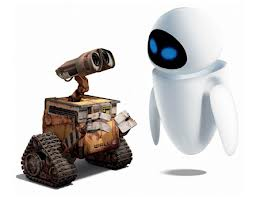
\includegraphics[scale=0.7, bb=0 0 256 197]{./Figuras/robot.jpg}
      \caption[Exemplo de figura com legenda.]{Exemplo de figura com legenda \cite{ref_2}.}
      \label{fig:exemplo}
  \end{center}
\end{figure}

Quando se representam as unidades deve existir o cuidado de deixar um espaço entre a grandeza e a unidade, devem ser inseparáveis no caso de mudança de linha.
\\Exemplos:
"... . . . . . . . . . . . . . . . cada iteração tem a duração de 22 ms..."(errado) ou "... ou 22ms..." (errado).\\
".... cada iteração tem a duração de \mbox{22 ms}..." (correcto)

Sempre que sejam escritas equações deve ser utilizado o ambiente adequado para que estas sejam numeradas automaticamente e se possam referenciar no texto. Exemplo disto é a equação \ref{nota_final}, utilizada para determinação da nota final.

\begin{equation}
 N_{f} = A \times R_{ar} + B \times R_{rp} + C \times R_{rf}
 \label{nota_final}
\end{equation}

\section{Enquadramento e Motivação}

Contextualizar o trabalho, explicar onde este se enquadra nas actividades do LSA e/ou de determinado projecto.

\section{Cenários de aplicação}
Descrever algumas aplicações que justifiquem a necessidade de realizar o trabalho e como este pode contribuir para a melhoria do processo.

\section{Objectivos}
Apresentar a lista de objectivos que se pretendem alcançar.

\section{Estrutura do Relatório}
No capítulo x é ...


\newpage

As tabelas também devem ter uma legenda, mas antes da tabela como mostra o exemplo da tabela \ref{tab:exemplo} e não devem ser utilizadas linhas verticais.

\begin{table}[h!]
\begin{center}
    \caption{Exemplo de tabela com legenda.}
    \begin{tabular}{lll}\hline
      1 & 2 & 3\\\hline
      4 & 5 & 6\\\hline
      7 & 8 & 9\\\hline
    \end{tabular}
    \label{tab:exemplo}
\end{center}
\end{table}
